\documentclass[11pt, oneside]{article}   	% use "amsart" instead of "article" for AMSLaTeX format
\usepackage{geometry}                		% See geometry.pdf to learn the layout options. There are lots.
\geometry{letterpaper}                   		% ... or a4paper or a5paper or ... 
%\geometry{landscape}                		% Activate for for rotated page geometry
%\usepackage[parfill]{parskip}    		% Activate to begin paragraphs with an empty line rather than an indent
\usepackage{graphicx}				% Use pdf, png, jpg, or eps� with pdflatex; use eps in DVI mode
								% TeX will automatically convert eps --> pdf in pdflatex		
\usepackage{amssymb}
\usepackage{amsmath}
\usepackage{parskip}
\usepackage{color}
\usepackage{hyperref}

\title{Kirchhoff}
%\author{The Author}
%\section{}
%\subsection*{}
\date{}							% Activate to display a given date or no date

\graphicspath{{/Users/telliott_admin/Dropbox/Tex/png/}}
% \begin{center} 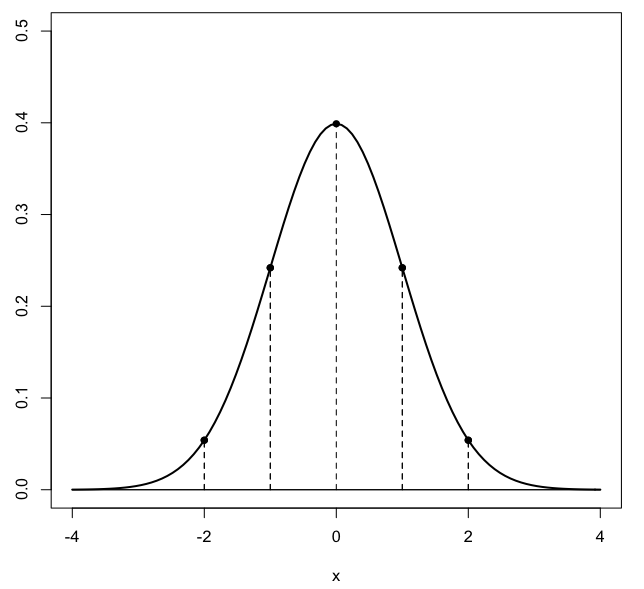
\includegraphics [scale=0.4] {gauss3.png} \end{center}
\begin{document}
\maketitle
\Large
Here is a circuit problem from Fitzpatrick.
\begin{center} 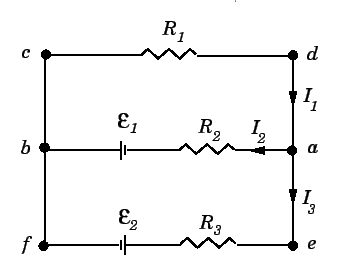
\includegraphics [scale=0.6] {circuit1.png} \end{center}
The resistances are given as $R_1=100 \Omega$, $R_2=10 \Omega$, and $R_1=5 \Omega$. The voltages are given as $\epsilon_1 = 12 V$ and $\epsilon_2 = 6 V$.
The directions for the currents are shown.  The equations we have are then
\[ I_1 = I_2 + I_3 \]
from the junction rule (current in equals current out).  Then, clockwise around the loop containing $R1$ and $R2$ (the high voltage side of $\epsilon_1$ is on the left
\[ -I_2 R_2 + \epsilon_1 + I_1 R_1 = 0 \]
The other loop we will use contains $R_2$ and $R_3$.
\[ -I_3 R_3 - \epsilon_2 - \epsilon_1 + I_2 R_2 = 0 \]
Solution.
Start by substituting into the second equation from the first
\[ -I_2 R_2 + \epsilon_1 + I_2 R_1 + I_3 R_1 = 0 \]
and rearrange
\[ I_2 (R_1-R_2) + \epsilon_1 + I_3 R_1 = 0 \]
Our plan is to remove $I_3$.  Get equation 3 together with the above, and move the $\epsilon$'s to the other side in both
\[ I_2 (R_1-R_2) + I_3 R_1 = - \epsilon_1 \]
\[ I_2 R_2 - I_3 R_3 = \epsilon_1 + \epsilon_2 \]
It's clear what to do, just a bit of a pain.
\[ \frac{I_2 (R_1-R_2)}{R_1} + I_3 = -\frac{\epsilon_1}{R_1} \]
\[ \frac{I_2 R_2}{R_3} - I_3 = \frac{\epsilon_1 + \epsilon_2}{R_3} \]
So
\[ \frac{I_2 (R_1-R_2)}{R_1} + \frac{I_2 R_2}{R_3} = -\frac{\epsilon_1}{R_1} + \frac{\epsilon_1 + \epsilon_2}{R_3} \]
The coefficients for $I_2$ are
\[ 0.9 + 2 = 2.9 \]
On the right-hand side we have
\[ -0.12 + 3.6 = 3.48 \]
So we calculate $I_2 = 3.48/2.9 = 1.2$.  From the second equation at the top we have
\[ -1.2 R_2 + \epsilon_1 + I_1 R_1 = 0 \]
\[ -1.2 (10) + 12 + I_1 R_1 = 0 \]
Notice:  it doesn't matter what $R_1$ is.  $I_1$ must equal $0$.  And then $I_3 = - I_2$.
Alternatively you can just plug the numbers into an online solver like this one:

\large
\url{http://www.gregthatcher.com/Mathematics/GaussJordan.aspx}

\begin{center} 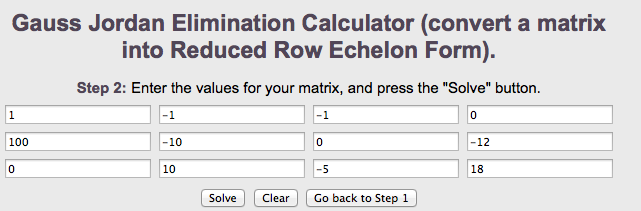
\includegraphics [scale=0.6] {input_K.png} \end{center}
\begin{center} 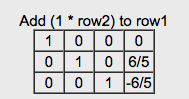
\includegraphics [scale=0.6] {output_K.png} \end{center}

\Large
The solver shows all the steps, but I didn't keep that part.

\end{document}  